\chapter{Resultados e Discussões}\label{cap:resultados}

Este capítulo apresenta e discute os resultados obtidos para as quatro
métricas definidas na Seção~\ref{sec:metricas}: taxa máxima de
amostragem sustentada (M1, Seção~\ref{sec:res-m1}), \emph{jitter} de
amostragem (M2, Seção~\ref{sec:res-m2}), perda de amostras em captura
contínua (M3, Seção~\ref{sec:res-m3}) e ocupação de \ac{CPU} (M4,
Seção~\ref{sec:res-m4}). O capítulo
encerra com uma síntese (Seção~\ref{sec:res-sintese}) que confronta os
resultados com o comportamento esperado de cada arquitetura
(Capítulo~\ref{cap:fundamentacao}).

\section{Visão geral}

O Quadro~\ref{qua:metricas} resume as quatro métricas avaliadas, a unidade
em que cada uma é reportada, o instrumento que a fornece e as equações que a
definem na Seção~\ref{sec:metricas}.

\begin{quadro}[H]
  \centering
  \caption{Resumo das métricas de comparação.}
  \label{qua:metricas}
  \begin{tabularx}{\linewidth}{|l|>{\raggedright\arraybackslash}p{2.9cm}|>{\raggedright\arraybackslash}p{2.4cm}|>{\raggedright\arraybackslash}X|l|}
    \hline
    \textbf{\#} & \textbf{Métrica}            & \textbf{Unidade}         & \textbf{Instrumento principal} & \textbf{Eq.} \\ \hline
    M1          & Taxa máxima sustentada      & MSa/s                     & Onda de referência + contagem de bordas (analisador lógico) & \ref{eq:m1-integra}, \ref{eq:m1-fmax} \\ \hline
    M2          & \emph{Jitter} de amostragem & ns ($\sigma$, p-p)       & Onda de referência + analisador lógico & \ref{eq:m2-periodo}--\ref{eq:jitter-exc} \\ \hline
    M3          & Perda em captura contínua   & \% amostras; lacunas/min & Onda de referência + detecção de lacunas e abortos & \ref{eq:m3-fracao}, \ref{eq:m3-lacuna} \\ \hline
    M4          & Ocupação de \acs{CPU}             & \% de ciclos ocupados    & Contador de ciclos \acs{DWT} & \ref{eq:m4-ocupacao} \\ \hline
  \end{tabularx}
  \fonte{Autoria própria.}
\end{quadro}

Em todas as figuras, cada ponto é a média das $N = 30$ repetições da
condição, e a faixa sombreada e as barras vão do menor ao maior valor
observado entre as repetições; o Firmware A é
representado em azul com linha contínua e círculos, e o Firmware B em laranja
com linha tracejada e quadrados. Nas tabelas, $p_{\mathrm{Holm}}$ é o p-valor
do teste de Mann--Whitney U ajustado por Holm--Bonferroni dentro da família
da métrica, e $r$ é a correlação \emph{rank-biserial}, com $r > 0$ indicando
valores maiores em B (Seção~\ref{sec:analise-estatistica}).

As condições de cada ensaio (sinal de 100\,kHz no canal D3, 4 e 12 canais
habilitados em M1--M3, janela de 0,2\,s em M1 e M2, captura de 60\,s em M3)
estão descritas na Seção~\ref{sec:metricas}.

\section{M1: Taxa máxima de amostragem sustentada}\label{sec:res-m1}

\subsection{Resultado}

O ensaio usou onda quadrada de 100\,kHz ($f_{sig} = 99{\,}999{,}83$\,Hz
segundo o analisador de referência), de modo que a varredura começa em $4 f_{sig} \approx
400$\,kS/s e prossegue em passos logarítmicos até a primeira taxa em que
alguma repetição falha. A Tabela~\ref{tab:m1-resumo} e a
Figura~\ref{fig:m1-integras} resumem o resultado.

\begin{table}[H]
  \centering
  \caption{M1: repetições íntegras e bordas contadas por taxa.}
  \label{tab:m1-resumo}
  \small
  \begin{tabular}{@{}llrrrr@{}}
    \toprule
    \textbf{Firmware} & \textbf{Canais} & \textbf{Taxa (kS/s)} &
    \textbf{Íntegras} & \textbf{Bordas \acs{DAQ} (mediana)} &
    \textbf{Excesso} \\
    \midrule
    A & 4  & 525,5    & 30/30 & 19\,999 & $-1$ \\
    A & 4  & 774,6    & 30/30 & 19\,999 & $-1$ \\
    A & 4  & 1\,141,7 & 30/30 & 19\,999 & $-1$ \\
    A & 4  & 1\,682,7 & 30/30 & 19\,999 & $-1$ \\
    A & 4  & 2\,480,2 & 30/30 & 20\,000 & $0$  \\
    A & 4  & 3\,655,6 & 30/30 & 20\,000 & $0$  \\
    A & 4  & 5\,388,0 & 0/30  & ---     & ---  \\
    A & 12 & 525,5    & 30/30 & 19\,999 & $-1$ \\
    A & 12 & 774,6    & 30/30 & 19\,999 & $-1$ \\
    A & 12 & 1\,141,7 & 30/30 & 20\,000 & $0$  \\
    A & 12 & 1\,682,7 & 30/30 & 19\,999 & $-1$ \\
    A & 12 & 2\,480,2 & 30/30 & 20\,000 & $0$  \\
    A & 12 & 3\,655,6 & 30/30 & 20\,000 & $0$  \\
    A & 12 & 5\,388,0 & 0/30  & ---     & ---  \\
    \midrule
    B & 4  & 525,5    & 30/30 & 19\,999 & $-1$  \\
    B & 4  & 774,6    & 30/30 & 20\,000 & $0$   \\
    B & 4  & 1\,141,7 & 30/30 & 20\,008 & $+8$  \\
    B & 4  & 1\,682,7 & 30/30 & 20\,010 & $+10$ \\
    B & 4  & 2\,480,2 & 30/30 & 20\,008 & $+8$  \\
    B & 4  & 3\,655,6 & 0/30  & 20\,028 & $+28$ \\
    B & 12 & 525,5    & 30/30 & 20\,001 & $+1$  \\
    B & 12 & 774,6    & 30/30 & 20\,000 & $0$   \\
    B & 12 & 1\,141,7 & 30/30 & 20\,003 & $+3$  \\
    B & 12 & 1\,682,7 & 30/30 & 20\,003 & $+3$  \\
    B & 12 & 2\,480,2 & 30/30 & 20\,005 & $+5$  \\
    B & 12 & 3\,655,6 & 0/30  & 20\,029 & $+29$ \\
    \bottomrule
  \end{tabular}
  \fonte{Autoria própria.}
  \nota{medianas de 30 repetições; janela de 0,2\,s; a referência registra 20\,000 bordas de subida por janela; excesso = bordas do DAQ $-$ bordas da referência. Em A a 5\,388,0\,kS/s, a captura é abortada pelo firmware.}
\end{table}

\begin{figure}[htbp]
  \centering
  \caption{M1: repetições íntegras por taxa de amostragem.}
  \label{fig:m1-integras}
  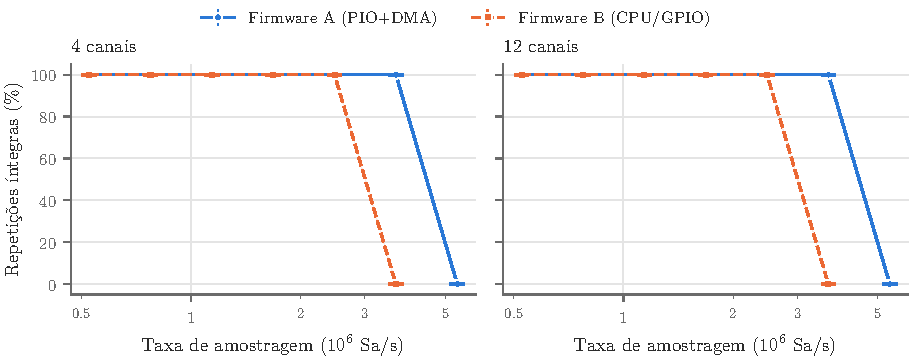
\includegraphics[width=\linewidth]{Cap04/img/m1_integras.pdf}
  \fonte{Autoria própria.}
\end{figure}

Pelo critério da Seção~\ref{sec:metricas} (tolerância de 0,1\,\% na
contagem), a taxa máxima sustentada do Firmware A é 3\,655,6\,kS/s e a do
Firmware B é 2\,480,2\,kS/s, tanto com 4 quanto com 12 canais. Os dois
firmwares, porém, falham de modos diferentes. Em A, a contagem de bordas
coincide com a da referência, a menos do corte da janela ($\pm 1$ borda),
em todas as repetições até 3\,655,6\,kS/s; na taxa seguinte, o firmware
detecta o transbordamento do \emph{buffer} e aborta a captura com o
marcador \texttt{!!!} do protocolo depois de entregar um único
\emph{buffer} de 1\,024 amostras. Em B, a captura nunca é abortada, mas o
\ac{DAQ} registra mais bordas do que a referência, e o excesso cresce com a taxa
(Figura~\ref{fig:m1-excesso}): a contagem é exata até 774,6\,kS/s, passa
a ter de 3 a 10 bordas a mais a partir de 1\,141,7\,kS/s, ainda dentro da
tolerância de 20 bordas, e salta para cerca de 28 bordas em
3\,655,6\,kS/s, quando todas as repetições falham.

\begin{figure}[htbp]
  \centering
  \caption{M1: excesso de bordas do DAQ em relação à referência.}
  \label{fig:m1-excesso}
  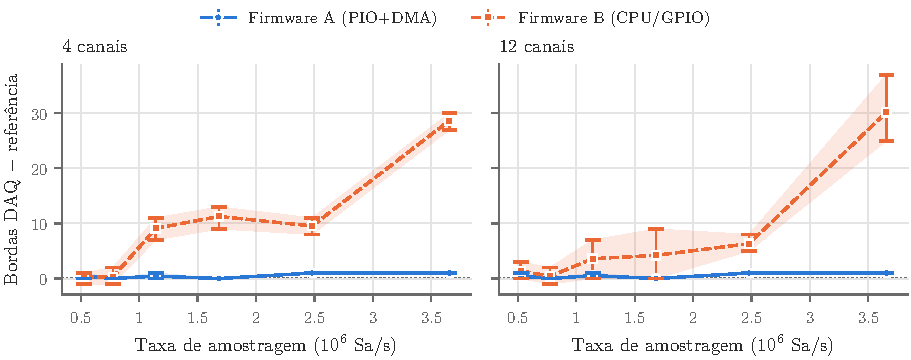
\includegraphics[width=\linewidth]{Cap04/img/m1_excesso_bordas.pdf}
  \fonte{Autoria própria.}
  \nota{repetições abortadas excluídas.}
\end{figure}

Bordas \emph{a mais} não podem vir de amostras perdidas em sequência
contínua; indicam que as amostras entregues cobrem um intervalo de tempo
maior que o nominal, isto é, que a amostragem foi interrompida e retomada
sem que o fluxo sinalizasse a interrupção. Uma pausa mais curta que meio
período do sinal não apaga bordas, mas desloca as seguintes; cada retomada
ocorre em fase arbitrária da onda, e o acúmulo dessas pausas faz a janela
de amostras se estender além de 0,2\,s e conter bordas extras. Esse é o
comportamento esperado de B quando o laço de amostragem é atrasado pelo
envio do bloco anterior. Se o critério de tolerância fosse reduzido a
$\pm 2$ bordas, suficiente para absorver o corte da janela, a taxa
sustentada de A não mudaria, enquanto a de B cairia para 774,6\,kS/s.

A comparação estatística usa a contagem de bordas de cada repetição nas
doze condições medidas pelos dois firmwares, de 525,5 a 3\,655,6\,kS/s
(Tabela~\ref{tab:m1-estat}). A partir de 1\,141,7\,kS/s, B conta mais
bordas que A em todas as condições, com separação completa ou quase
completa entre as repetições ($r \ge +0{,}90$): a diferença de medianas
vai de 2 a 12 bordas até 2\,480,2\,kS/s e chega a 27 a 30 bordas em
3\,655,6\,kS/s. Em 525,5 e 774,6\,kS/s a diferença é de no máximo duas
bordas e só é significativa em 525,5\,kS/s com 12 canais, ainda assim
dentro do corte da janela e sem relevância prática.

\begin{table}[H]
  \centering
  \caption{M1: comparação estatística da contagem de bordas (B $-$ A).}
  \label{tab:m1-estat}
  \begin{tabular}{@{}rrrrr@{}}
    \toprule
    \textbf{Canais} & \textbf{Taxa (kS/s)} & $\boldsymbol{r}$ &
    $\boldsymbol{p_{\mathrm{Holm}}}$ & \textbf{IC 95\,\% (bordas)} \\
    \midrule
    4 & 525{,}5 & $-0{,}14$ & $3{,}1 \times 10^{-1}$ & $[-1; 1]$ \\
    4 & 774{,}6 & $+0{,}20$ & $2{,}6 \times 10^{-1}$ & $[0; 1]$ \\
    4 & 1\,141{,}7 & $+1{,}00$ & $8{,}5 \times 10^{-11}$ & $[8; 10]$ \\
    4 & 1\,682{,}7 & $+1{,}00$ & $8{,}2 \times 10^{-12}$ & $[11; 12]$ \\
    4 & 2\,480{,}2 & $+1{,}00$ & $8{,}2 \times 10^{-12}$ & $[8; 9]$ \\
    4 & 3\,655{,}6 & $+1{,}00$ & $8{,}2 \times 10^{-12}$ & $[27; 28]$ \\
    \midrule
    12 & 525{,}5 & $+0{,}63$ & $2{,}9 \times 10^{-5}$ & $[0; 2]$ \\
    12 & 774{,}6 & $+0{,}27$ & $1{,}3 \times 10^{-1}$ & $[0; 1]$ \\
    12 & 1\,141{,}7 & $+0{,}93$ & $1{,}2 \times 10^{-9}$ & $[2; 4]$ \\
    12 & 1\,682{,}7 & $+0{,}90$ & $3{,}2 \times 10^{-10}$ & $[3; 6]$ \\
    12 & 2\,480{,}2 & $+1{,}00$ & $8{,}2 \times 10^{-12}$ & $[5; 6]$ \\
    12 & 3\,655{,}6 & $+1{,}00$ & $9{,}3 \times 10^{-12}$ & $[28; 30]$ \\
    \bottomrule
  \end{tabular}
  \fonte{Autoria própria.}
  \nota{$n = 30$ repetições por firmware; Mann--Whitney U com correção de Holm--Bonferroni dentro da família da métrica; $r$: correlação \emph{rank-biserial} ($r > 0$: mais bordas em B); IC 95\,\% da diferença de medianas (B $-$ A) por \emph{bootstrap}.}
\end{table}

\subsection{Discussão}

O resultado confirma a vantagem esperada do hardware dedicado
(Seção~\ref{sec:polling}): A sustenta uma taxa cerca de 1,5 vez maior que
B pelo critério de 0,1\,\%, e 4,7 vezes maior pelo de $\pm 2$ bordas. A
diferença qualitativa pesa tanto quanto a quantitativa: dentro da faixa
sustentada A entrega exatamente o sinal da referência e, fora dela,
recusa a captura explicitamente; B degrada em silêncio, entregando uma
janela completa cuja escala de tempo não corresponde à real.

Nenhum dos dois tetos vem do amostrador. O de B não é dado pelo custo do
laço, medido pelo próprio firmware em $C_{iter} = 35$ ciclos por amostra
com o contador \ac{DWT}, o que permitiria $\approx 4{,}29$\,MS/s pela
Equação~\ref{eq:fsmax}; B falha em 85\,\% desse teto, por causa das
pausas silenciosas que surgem a partir de $\approx 1{,}1$\,MS/s e crescem
abruptamente acima de 2,5\,MS/s. O de A não vem do \ac{PIO}, capaz de
amostrar a dezenas de MS/s, e sim do caminho que consome as amostras: a
\ac{CPU} ainda codifica cada amostra em \ac{RLE} (Seção~\ref{sec:res-m4})
e, quando não acompanha a taxa, o par de \emph{buffers} do \ac{DMA}, de
1\,024 amostras cada, se esgota. Como o par cobre apenas
$\approx 0{,}4$\,ms a 5\,MS/s, basta um atraso transitório: na captura
contínua (Seção~\ref{sec:res-m3}), a 5\,236,7\,kS/s a maioria das
capturas aborta logo após os dois primeiros \emph{buffers}, no início da
transferência \ac{USB}. A vantagem arquitetural de A só se converte em
taxa maior se o processamento do fluxo também sair da \ac{CPU}, ou se a
fila entre o \ac{DMA} e a \ac{CPU} for mais profunda.

Que o limite de A esteja no consumo das amostras, e não na arquitetura
\ac{PIO}+\ac{DMA}, é confirmado por projetos de código aberto: o analisador
de \citeonline{gusmanb_logicanalyzer}, com o mesmo encadeamento \ac{PIO}--\ac{DMA},
anuncia 100\,MS/s no RP2040 porque não transmite durante a captura, modo em
que o \ac{DMA} grava em um \emph{buffer} circular na \ac{SRAM} e o envio ao
\emph{host} só começa depois da janela, em troca de capturas limitadas à
memória. As duas abordagens são pontos distintos de uma mesma troca entre
taxa de amostragem e duração da captura, e não arquiteturas com
capacidades diferentes de amostragem.

Cabe registrar que a versão inicial do Firmware A rearmava o \ac{PIO} e a
\ac{DMA} a cada 1\,024 amostras nas capturas com disparo, deixando uma
lacuna não sinalizada de $\approx 1{,}5$\,\textmu s por bloco; o efeito
era o mesmo excesso de bordas observado em B e limitava a taxa sustentada
a 774,6\,kS/s. A correção passou a usar o \ac{DMA} encadeado em
\emph{ping-pong} também com disparo, e os resultados desta seção
referem-se à versão corrigida.

\section{M2: \emph{Jitter} de amostragem}\label{sec:res-m2}

\subsection{Resultado}

O ensaio usou a mesma onda quadrada de 100\,kHz da M1 (a referência
registra 19\,999 períodos por janela), janela de 0,2\,s após o disparo e
taxas de 2,0 a 4,05\,MS/s, o teto aceito pelo Firmware B. O período é medido
em amostras entre bordas de subida consecutivas e convertido para tempo pela
taxa solicitada. Um primeiro ensaio com onda de 1\,MHz foi descartado: nessa
frequência a codificação \ac{RLE} quase não compacta o fluxo, a demanda supera a
vazão do \ac{USB} Full-Speed (Seção~\ref{sec:res-m3}), e o Firmware A aborta a
captura enquanto o Firmware B entrega a janela com amostras faltando, de
modo que a medida passaria a refletir o barramento e não o amostrador.

O desvio-padrão medido $\sigma$ é confrontado com o limite de quantização
$\sigma_q$ de um amostrador ideal (Equação~\ref{eq:jitter-quant}), e apenas
o excedente $\sigma_{exc}$ (Equação~\ref{eq:jitter-exc}) é atribuído à
instabilidade do instante de amostragem. A Tabela~\ref{tab:m2-jitter} e a
Figura~\ref{fig:m2-std} trazem os valores medidos.

\begin{table}[H]
  \centering
  \caption{M2: desvio-padrão do período e diferença na contagem de períodos.}
  \label{tab:m2-jitter}
  \begin{tabular}{@{}rrrrrrrr@{}}
    \toprule
    & & & \multicolumn{2}{c}{$\boldsymbol{\sigma_B}$ \textbf{(ns)}} &
    & \multicolumn{2}{c}{$\boldsymbol{\Delta n_B}$} \\
    \cmidrule(lr){4-5}\cmidrule(l){7-8}
    \textbf{Taxa (MS/s)} & $\boldsymbol{\sigma_q}$ \textbf{(ns)} &
    $\boldsymbol{\sigma_A}$ \textbf{(ns)} & \textbf{4 can.} & \textbf{12 can.} &
    $\boldsymbol{\Delta n_A}$ & \textbf{4 can.} & \textbf{12 can.} \\
    \midrule
    2,00 &  15,8 &  12,2 & 183,9 & 216,8 & $-1$ & $+5$    & $+17$   \\
    2,25 & 222,3 & 222,3 & 247,3 & 295,8 & $-1$ & $-1$    & $+17{,}5$ \\
    2,53 & 181,8 & 181,7 & 263,3 & 271,1 & $-1$ & $-4{,}5$ & $+3$    \\
    2,85 & 175,2 & 175,2 & 263,0 & 205,0 & $-1$ & $+17$   & $+8$    \\
    3,20 &  36,2 &  36,7 & 252,6 & 293,1 & $-2$ & $+9$    & $+27{,}5$ \\
    3,60 &  25,6 &  22,5 & 330,2 & 309,0 & $0$  & $+18$   & $+20$   \\
    4,05 & 123,5 & 123,5 & 418,4 & 333,3 & $-2$ & $+42$   & $+8$    \\
    \bottomrule
  \end{tabular}
  \fonte{Autoria própria.}
  \nota{medianas de 30 repetições; $\sigma_q$: limite de quantização (Equação~\ref{eq:jitter-quant}); $\Delta n$: períodos do DAQ $-$ períodos da referência. Valores de A iguais com 4 e 12 canais.}
\end{table}

\begin{figure}[htbp]
  \centering
  \caption{M2: desvio-padrão do período por taxa de amostragem.}
  \label{fig:m2-std}
  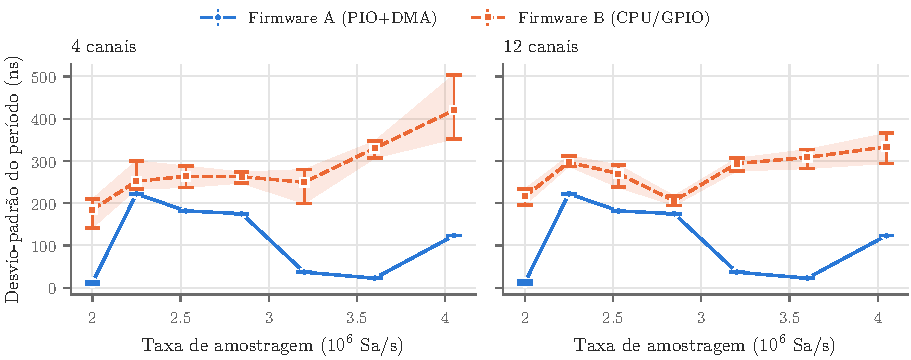
\includegraphics[width=\linewidth]{Cap04/img/m2_jitter_std.pdf}
  \fonte{Autoria própria.}
\end{figure}

O desvio-padrão do Firmware A coincide com o limite de quantização em toda
a faixa, a menos de 3,6\,ns (no máximo, um excedente de 5,9\,ns em
3,20\,MS/s), e acompanha inclusive as oscilações de $\sigma_q$ com a taxa;
as diferenças estão dentro da incerteza com que $f_{sig}$ é conhecida, o
que explica $\sigma_A$ ficar ligeiramente abaixo de $\sigma_q$ em algumas
taxas, já que $\sigma_q$ é calculado com a frequência aferida, e não com a
real.
As 30 repetições de A são praticamente idênticas, de modo que, nas figuras,
o intervalo entre o mínimo e o máximo de A fica menor que o próprio
marcador. O Firmware B fica acima de $\sigma_q$ em todas as condições, com
excedente de 106 a 400\,ns, o equivalente a 16 a 60 ciclos de \ac{CPU} a
150\,MHz, e com variação visível entre repetições. O valor pico a pico do
período separa ainda mais os dois: de 0,25 a 1,0\,\textmu s em A e de 6,3 a
13,3\,\textmu s em B, isto é, B registra intervalos entre bordas que
chegam a quase dois períodos do sinal.

A contagem de períodos (Figura~\ref{fig:m2-perdidos}) repete o padrão da
M1. Em A, a diferença para a referência fica entre $-2$ e 0, apenas o corte
da janela. Em B, a captura contém em geral \emph{mais} períodos que a
referência, até 42 a mais em 4,05\,MS/s com 4 canais (0,21\,\% da janela).

\begin{figure}[htbp]
  \centering
  \caption{M2: períodos ausentes em relação à referência.}
  \label{fig:m2-perdidos}
  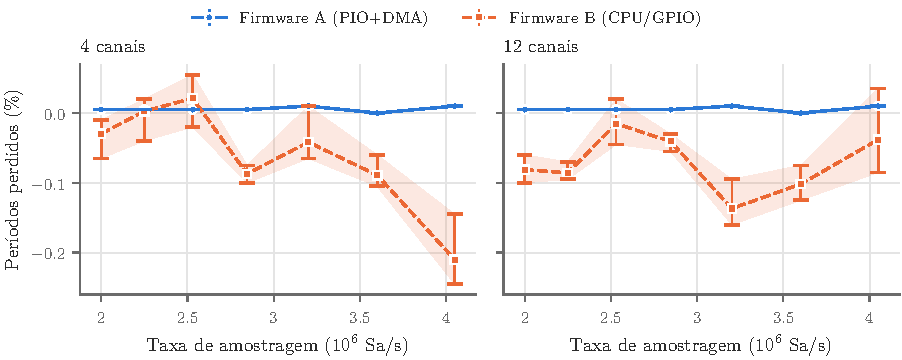
\includegraphics[width=\linewidth]{Cap04/img/m2_periodos_perdidos.pdf}
  \fonte{Autoria própria.}
  \nota{em percentual da janela; valores negativos indicam períodos a mais (sinal oposto ao de $\Delta n$ na Tabela~\ref{tab:m2-jitter}).}
\end{figure}

A comparação estatística cobre as 14 condições (sete taxas $\times$ duas
contagens de canais) e três medidas: o desvio-padrão do período, seu
valor pico a pico e a diferença na contagem de períodos
(Tabela~\ref{tab:m2-estat}). Nas duas primeiras, a separação é completa
em todas as condições ($r = +1{,}00$;
$p_{\mathrm{Holm}} \le 1{,}6 \times 10^{-10}$), com B acima de A por 20
a 311\,ns no desvio-padrão e por 5,3 a 13,1\,\textmu s no pico a pico.
Na contagem de períodos, B conta mais que A em 12 das 14 condições; a
diferença não é significativa em 2,25\,MS/s com 4 canais e se inverte
em 2,53\,MS/s com 4 canais, em até 6,5 períodos.

\begin{table}[H]
  \centering
  \caption{M2: comparação estatística das medidas de período (B $-$ A).}
  \label{tab:m2-estat}
  \resizebox{\linewidth}{!}{%
  \begin{tabular}{@{}rrrrrrr@{}}
    \toprule
    & & \multicolumn{2}{c}{\textbf{IC 95\,\% da diferença}} &
    \multicolumn{3}{c}{\textbf{Contagem de períodos} $\boldsymbol{\Delta n}$} \\
    \cmidrule(lr){3-4}\cmidrule(l){5-7}
    \textbf{Canais} & \textbf{Taxa (MS/s)} & $\boldsymbol{\sigma}$ \textbf{(ns)} &
    \textbf{pico a pico (\textmu s)} & $\boldsymbol{r}$ &
    $\boldsymbol{p_{\mathrm{Holm}}}$ & \textbf{IC 95\,\%} \\
    \midrule
    4 & 2{,}00 & $[166{,}4; 177{,}0]$ & $[10{,}2; 11{,}5]$ & $+1{,}00$ & $1{,}3 \times 10^{-11}$ & $[5{,}5; 7{,}5]$ \\
    4 & 2{,}25 & $[20{,}3; 34{,}3]$ & $[10{,}2; 10{,}7]$ & $+0{,}03$ & $8{,}1 \times 10^{-1}$ & $[-1{,}0; 1{,}0]$ \\
    4 & 2{,}53 & $[74{,}0; 90{,}1]$ & $[11{,}1; 11{,}5]$ & $-0{,}50$ & $7{,}0 \times 10^{-4}$ & $[-6{,}5; -1{,}0]$ \\
    4 & 2{,}85 & $[85{,}8; 89{,}8]$ & $[10{,}2; 10{,}9]$ & $+1{,}00$ & $1{,}3 \times 10^{-11}$ & $[18{,}0; 19{,}0]$ \\
    4 & 3{,}20 & $[208{,}3; 219{,}0]$ & $[10{,}9; 11{,}9]$ & $+0{,}97$ & $2{,}2 \times 10^{-11}$ & $[9{,}0; 12{,}0]$ \\
    4 & 3{,}60 & $[304{,}6; 310{,}8]$ & $[11{,}7; 11{,}9]$ & $+1{,}00$ & $1{,}3 \times 10^{-11}$ & $[17{,}0; 19{,}0]$ \\
    4 & 4{,}05 & $[281{,}8; 308{,}7]$ & $[11{,}4; 12{,}0]$ & $+1{,}00$ & $1{,}3 \times 10^{-11}$ & $[42{,}0; 47{,}0]$ \\
    \midrule
    12 & 2{,}00 & $[200{,}6; 210{,}2]$ & $[10{,}0; 11{,}0]$ & $+1{,}00$ & $1{,}3 \times 10^{-11}$ & $[17{,}0; 18{,}0]$ \\
    12 & 2{,}25 & $[70{,}9; 76{,}8]$ & $[10{,}2; 11{,}3]$ & $+1{,}00$ & $1{,}3 \times 10^{-11}$ & $[18{,}0; 19{,}0]$ \\
    12 & 2{,}53 & $[82{,}8; 94{,}6]$ & $[11{,}1; 11{,}5]$ & $+0{,}87$ & $2{,}2 \times 10^{-9}$ & $[3{,}0; 5{,}5]$ \\
    12 & 2{,}85 & $[28{,}1; 33{,}0]$ & $[5{,}3; 6{,}7]$ & $+1{,}00$ & $1{,}3 \times 10^{-11}$ & $[9{,}0; 10{,}0]$ \\
    12 & 3{,}20 & $[252{,}3; 262{,}8]$ & $[11{,}2; 11{,}6]$ & $+1{,}00$ & $1{,}3 \times 10^{-11}$ & $[28{,}0; 31{,}5]$ \\
    12 & 3{,}60 & $[281{,}8; 292{,}3]$ & $[12{,}5; 13{,}1]$ & $+1{,}00$ & $1{,}3 \times 10^{-11}$ & $[19{,}0; 22{,}0]$ \\
    12 & 4{,}05 & $[200{,}9; 220{,}8]$ & $[12{,}3; 12{,}8]$ & $+0{,}93$ & $1{,}3 \times 10^{-10}$ & $[8{,}0; 12{,}5]$ \\
    \bottomrule
  \end{tabular}}
  \fonte{Autoria própria.}
  \nota{$n = 30$ repetições por firmware; IC 95\,\% da diferença de medianas (B $-$ A) por \emph{bootstrap}. Em $\sigma$ e no pico a pico, $r = +1{,}00$ e $p_{\mathrm{Holm}} \le 1{,}6 \times 10^{-10}$ em todas as condições.}
\end{table}

\subsection{Discussão}

O resultado confirma o esperado (Seção~\ref{sec:determinismo}): a
amostragem pela \ac{CPU} introduz uma instabilidade de período que o
\ac{PIO} não apresenta. No Firmware A, o instante de cada amostra é
fixado pelo divisor de clock da máquina de estados e não depende
de software; o desvio observado é exatamente o de quantização, e a
medida é repetível entre capturas. No Firmware B, o laço usa prazos
absolutos no contador \ac{DWT} e ainda assim acumula dezenas de ciclos de
\emph{jitter}, porque o custo de cada iteração varia com o caminho
tomado (armazenamento, troca de \emph{buffer}, verificação de parada),
com as interrupções atendidas durante o laço, entre elas as da pilha
\ac{USB}, e com as esperas da execução a partir da flash (\acs{XIP}) e
da arbitragem de barramento.

Esse \emph{jitter} de ciclo a ciclo, porém, não explica o pico a pico de
B nem os períodos a mais: ambos apontam o mecanismo já identificado na
M1, o laço interrompido e retomado sem que o fluxo sinalize a pausa.
Acumuladas ao longo da janela, essas pausas fazem as amostras entregues
cobrirem mais que 0,2\,s, daí os períodos a mais; uma pausa que cobre um
pulso inteiro funde dois períodos em um, daí os intervalos de quase dois
períodos. A variação dessas pausas entre repetições é o que produz a
dispersão de B nas figuras, ausente em A.

\section{M3: Captura contínua e perda de amostras}\label{sec:res-m3}

\subsection{Resultado}

O ensaio aplicou a onda de 100\,kHz ao canal D3 e manteve a captura
contínua por 60\,s em cada uma das 30 repetições, com taxas a partir de
1,09\,MS/s (abaixo dela, o período tem menos de oito amostras e a detecção
de lacunas perde sensibilidade). A perda é medida de duas formas: pela
fração de amostras entregues em relação às solicitadas no tempo de captura
($f_s \times 60$\,s) e pelo número de lacunas, detectadas quando o
intervalo entre bordas se desvia do período nominal. A varredura de cada
contagem de canais para na primeira taxa em que todas as repetições
abortam ou que o firmware recusa.

O Firmware A sustentou a captura contínua em todas as 30 repetições até
3,54\,MS/s, com 4 e com 12 canais, entregando 100\,\% das amostras e sem
nenhuma lacuna (Tabela~\ref{tab:m3-resumo} e
Figuras~\ref{fig:m3-entregues} e~\ref{fig:m3-lacunas}). Em 5,24\,MS/s,
todas as repetições abortaram logo na partida, com a marca \texttt{!!!},
depois de entregar um ou dois \emph{buffers} de 1\,024 amostras
(Figura~\ref{fig:m3-abortadas}). O Firmware B recusa essa taxa na
configuração, por estar acima do teto do seu laço de amostragem, e não
abortou nenhuma captura nas taxas aceitas; em todas elas, porém, entregou
bem menos amostras do que o solicitado: de 75,7\,\% em 1,09\,MS/s a
57,3\,\% em 3,54\,MS/s, perda que cresce com a taxa e praticamente não
depende da contagem de canais.

\begin{table}[H]
  \centering
  \caption{M3: amostras entregues e lacunas em captura contínua de 60\,s.}
  \label{tab:m3-resumo}
  \begin{tabular}{@{}rrrrrrr@{}}
    \toprule
    & & \multicolumn{2}{c}{\textbf{Firmware A}} &
    \multicolumn{3}{c}{\textbf{Firmware B}} \\
    \cmidrule(lr){3-4}\cmidrule(l){5-7}
    \textbf{Canais} & \textbf{Taxa} & \textbf{Entregue} & \textbf{Lacunas} &
    \textbf{Entregue} & \textbf{Lacunas} & \textbf{Taxa efetiva} \\
    & (MS/s) & (\%) & & (\%) & & (MS/s) \\
    \midrule
    4  & 1,09 & 100,0 & 0 & 75,7 &  1\,774 & 0,83 \\
    4  & 1,62 & 100,0 & 0 & 71,2 & 10\,470 & 1,15 \\
    4  & 2,39 & 100,0 & 0 & 65,5 & 15\,398 & 1,57 \\
    4  & 3,54 & 100,0 & 0 & 58,5 & 63\,564 & 2,07 \\
    12 & 1,09 & 100,0 & 0 & 73,8 &  4\,789 & 0,81 \\
    12 & 1,62 & 100,0 & 0 & 69,5 &  8\,540 & 1,13 \\
    12 & 2,39 & 100,0 & 0 & 64,0 & 14\,882 & 1,53 \\
    12 & 3,54 & 100,0 & 0 & 57,3 & 69\,933 & 2,03 \\
    \bottomrule
  \end{tabular}
  \fonte{Autoria própria.}
  \nota{medianas de 30 repetições; taxa efetiva = amostras entregues / duração da captura.}
\end{table}

\begin{figure}[htbp]
  \centering
  \caption{M3: amostras entregues por taxa de amostragem.}
  \label{fig:m3-entregues}
  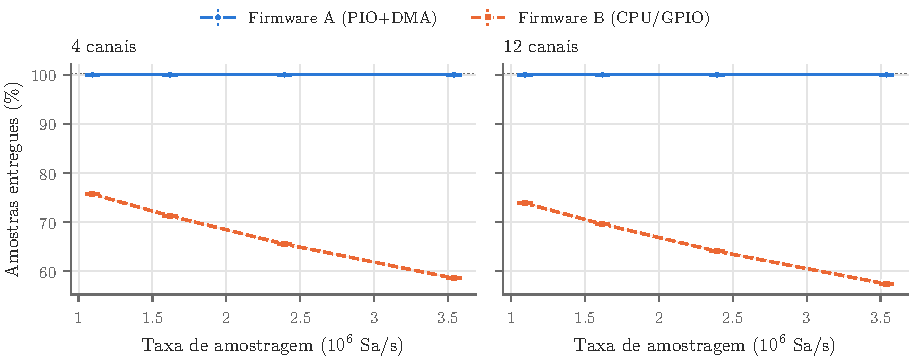
\includegraphics[width=\linewidth]{Cap04/img/m3_entregues.pdf}
  \fonte{Autoria própria.}
  \nota{em percentual das solicitadas; apenas condições sem aborto.}
\end{figure}

\begin{figure}[htbp]
  \centering
  \caption{M3: lacunas por minuto por taxa de amostragem.}
  \label{fig:m3-lacunas}
  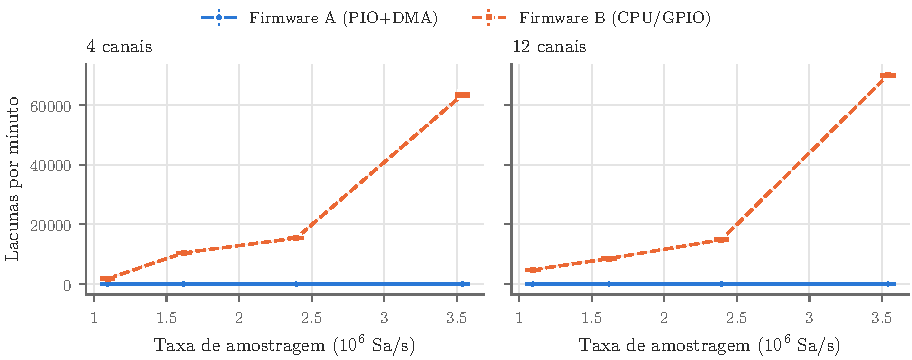
\includegraphics[width=\linewidth]{Cap04/img/m3_lacunas.pdf}
  \fonte{Autoria própria.}
  \nota{apenas condições sem aborto.}
\end{figure}

\begin{figure}[htbp]
  \centering
  \caption{M3: capturas abortadas por taxa de amostragem.}
  \label{fig:m3-abortadas}
  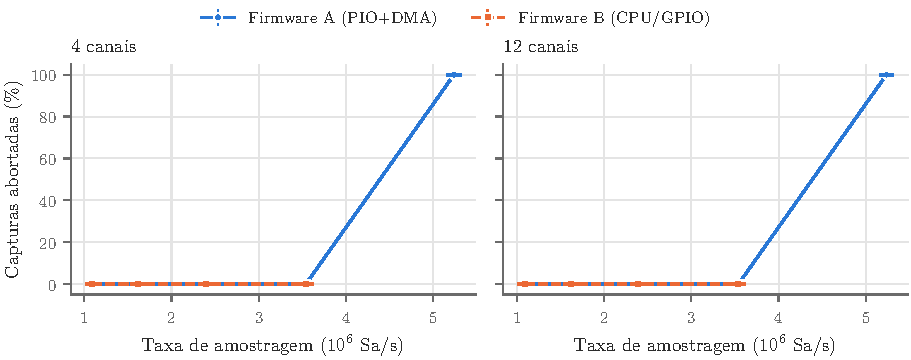
\includegraphics[width=\linewidth]{Cap04/img/m3_abortadas.pdf}
  \fonte{Autoria própria.}
\end{figure}

As duas medidas de perda de B devem ser lidas juntas. Como o sinal é
periódico, uma pausa que dure um número inteiro de períodos não altera o
intervalo entre bordas; a detecção enxerga apenas o resto da pausa em
relação ao período, e a lacuna detectada tem sempre menos de um período
(de 2 a 9 amostras, na mediana). O número de lacunas, de 1\,774 a 69\,933
por captura, é portanto um limite inferior do número de pausas, e o tamanho
das lacunas não mede a perda. A perda real é dada pela fração entregue: B
deixa de amostrar de 14 a 26\,s em cada captura de 60\,s, sem nenhuma
marca no fluxo que permita ao \emph{host} localizar esses trechos. As
lacunas de B não se concentram em nenhuma posição do bloco de $10^6$
amostras do modo contínuo (0,3\,\% delas nas primeiras 20 amostras), o que
as associa ao laço de amostragem, e não ao rearme de blocos.

Para separar o limite do barramento do limite do firmware, mediu-se
também a vazão \ac{USB} em captura contínua com sinal pouco compressível
(Figura~\ref{fig:usb-vazao}). O Firmware B satura o barramento em
$\approx 0{,}86$\,MB/s, 71\,\% do teto teórico do \ac{USB} Full-Speed
(1,216\,MB/s), e nesse regime entrega apenas 15 a 42\,\% das amostras
solicitadas. O Firmware A sustenta a captura sem perda enquanto a demanda
fica abaixo de $\approx 0{,}80$\,MB/s; acima de $\approx 0{,}92$\,MB/s,
ele aborta a captura em vez de descartar amostras.

\begin{figure}[htbp]
  \centering
  \caption{Vazão USB em captura contínua.}
  \label{fig:usb-vazao}
  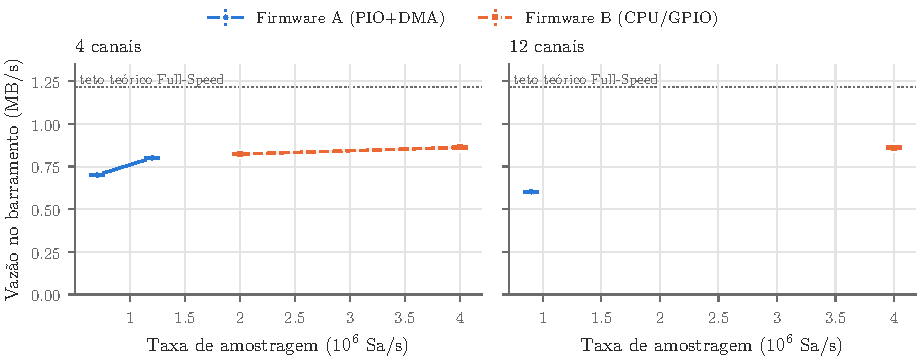
\includegraphics[width=\linewidth]{Cap04/img/usb_vazao.pdf}
  \fonte{Autoria própria.}
  \nota{apenas condições sem aborto; linha pontilhada: teto teórico do USB Full-Speed.}
\end{figure}

A comparação estatística usa as oito condições em que os dois firmwares
completaram a captura, quatro taxas $\times$ duas contagens de canais
(Tabela~\ref{tab:m3-estat}). Nas duas medidas, a separação é completa
em todas as repetições: B entrega uma fração menor das amostras
($r = -1{,}00$; $p_{\mathrm{Holm}} = 2{,}2 \times 10^{-10}$), de 24,3 a
42,7 pontos percentuais a menos, e apresenta mais lacunas
($r = +1{,}00$; $p_{\mathrm{Holm}} = 9{,}7 \times 10^{-12}$), de cerca
de 1\,800 a 70\,000 por captura. Os intervalos estreitos refletem a
baixa variação entre repetições, já que em cada condição a fração entregue
por B varia menos de 0,1 ponto percentual, isto é, a perda de B é
sistemática, e não ocasional.

\begin{table}[H]
  \centering
  \caption{M3: comparação estatística da perda de amostras (B $-$ A).}
  \label{tab:m3-estat}
  \begin{tabular}{@{}rrrr@{}}
    \toprule
    & & \multicolumn{2}{c}{\textbf{IC 95\,\% da diferença de medianas}} \\
    \cmidrule(l){3-4}
    \textbf{Canais} & \textbf{Taxa (MS/s)} &
    \textbf{Entregue (p.p.)} & \textbf{Lacunas} \\
    \midrule
    4 & 1{,}09 & $[-24{,}34; -24{,}34]$ & $[1\,748; 1\,818]$ \\
    4 & 1{,}62 & $[-28{,}79; -28{,}79]$ & $[10\,460; 10\,492]$ \\
    4 & 2{,}39 & $[-34{,}53; -34{,}53]$ & $[15\,388; 15\,410]$ \\
    4 & 3{,}54 & $[-41{,}49; -41{,}49]$ & $[63\,410; 63\,626]$ \\
    \midrule
    12 & 1{,}09 & $[-26{,}19; -26{,}19]$ & $[4\,766; 4\,822]$ \\
    12 & 1{,}62 & $[-30{,}46; -30{,}46]$ & $[8\,489; 8\,550]$ \\
    12 & 2{,}39 & $[-35{,}99; -35{,}99]$ & $[14\,869; 14\,896]$ \\
    12 & 3{,}54 & $[-42{,}68; -42{,}67]$ & $[69\,863; 70\,002]$ \\
    \bottomrule
  \end{tabular}
  \fonte{Autoria própria.}
  \nota{$n = 30$ repetições por firmware; IC por \emph{bootstrap}. Em todas as condições, $r = -1{,}00$ na fração entregue ($p_{\mathrm{Holm}} = 2{,}2 \times 10^{-10}$) e $r = +1{,}00$ nas lacunas ($p_{\mathrm{Holm}} = 9{,}7 \times 10^{-12}$).}
\end{table}

\subsection{Discussão}

O conflito entre amostrar e transmitir aparece apenas no Firmware B. Com
a onda de 100\,kHz, o fluxo compactado fica bem abaixo do teto do
\ac{USB} em toda a faixa, e A comprova isso ao entregar 100\,\% das
amostras até 3,54\,MS/s: a perda de B não vem do barramento, e sim da
disputa interna ao firmware. Em B, o laço de amostragem para enquanto um
bloco é entregue à pilha \ac{USB}, e o tempo dessas pausas cresce com a
taxa, de modo que a taxa efetiva sobe de 0,83 para apenas 2,07\,MS/s
enquanto a solicitada vai de 1,09 a 3,54\,MS/s. Em A, o \ac{DMA} continua amostrando
enquanto a \ac{CPU} transmite, e a fila de dois \emph{buffers} absorve a
variação do envio. A diferença qualitativa repete a da M1: A entrega um
fluxo sem perda dentro da faixa sustentada e aborta sinalizando fora
dela, pela mesma razão discutida na Seção~\ref{sec:res-m1} (a partida da
transferência \ac{USB} atrasa o consumo dos \emph{buffers}, e dois
\emph{buffers} cobrem menos de meio milissegundo a 5,24\,MS/s); B nunca
sinaliza e entrega, em toda a faixa, um fluxo que aparenta ser contínuo
mas em que um quarto a quase metade do tempo não foi amostrado.

Cabe registrar, como na M1, que a versão inicial do Firmware A rearmava
o \ac{PIO} e o \ac{DMA} a cada bloco de $10^6$ amostras do modo contínuo,
deixando cerca de uma lacuna silenciosa de 2,7 a 3,4\,\textmu s por
bloco, com 88,6\,\% delas nas primeiras 20 amostras. A correção passou a
armar o \ac{DMA} encadeado uma única vez por captura, e os resultados
desta seção referem-se à versão corrigida, que não apresentou nenhuma
lacuna em 240 capturas de 60\,s.

\section{M4: Ocupação de CPU}\label{sec:res-m4}

\subsection{Resultado}

A Figura~\ref{fig:m4-ocupacao} mostra a fração de ciclos em que a \ac{CPU}
esteve ocupada durante a captura, medida pelo contador \ac{DWT}, com a onda de
1\,MHz aplicada aos canais. A Tabela~\ref{tab:m4-ocupacao} traz valores
selecionados.

\begin{figure}[htbp]
  \centering
  \caption{M4: ocupação da CPU por taxa de amostragem.}
  \label{fig:m4-ocupacao}
  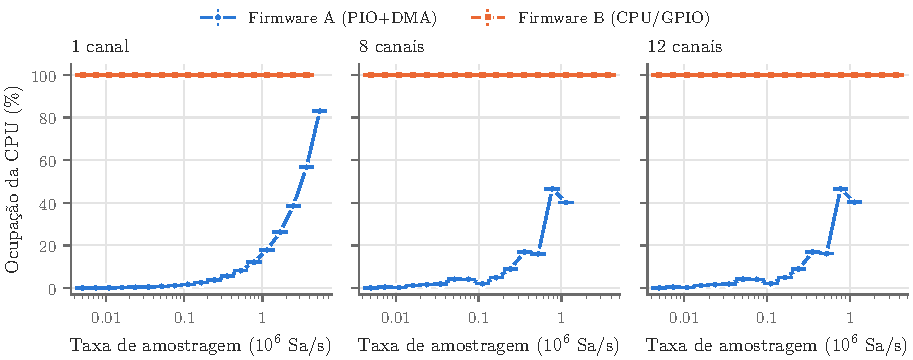
\includegraphics[width=\linewidth]{Cap04/img/m4_ocupacao.pdf}
  \fonte{Autoria própria.}
\end{figure}

\begin{table}[H]
  \centering
  \caption{M4: ocupação da CPU.}
  \label{tab:m4-ocupacao}
  \begin{tabular}{@{}rrrrr@{}}
    \toprule
    \textbf{Taxa (kS/s)} & \textbf{A, 1 canal} & \textbf{A, 8 canais} &
    \textbf{A, 12 canais} & \textbf{B (1, 8, 12 canais)} \\
    \midrule
    5,0      &  0,08 &  0,08 &  0,08 & 100,0 \\
    111,4    &  1,75 &  2,10 &  2,11 & 100,0 \\
    525,5    &  8,23 & 16,12 & 16,18 & 100,0 \\
    1\,141,7 & 17,84 & 40,16 & 40,26 & 100,0 \\
    3\,655,6 & 56,60 & ---   & ---   & 100,0 \\
    5\,388,0 & 82,95 & ---   & ---   & ---   \\
    \bottomrule
  \end{tabular}
  \fonte{Autoria própria.}
  \nota{em \%; medianas de 30 repetições.}
\end{table}

No Firmware A, a ocupação parte de 0,08\,\% e cresce com a taxa: 17,8\,\%
em 1,14\,MS/s com um canal e 83,0\,\% em 5,39\,MS/s, a maior taxa que
completou a captura. Com 8 e 12 canais, a ocupação é maior, até 46,6\,\%, e
as capturas abortam a partir de 1,68\,MS/s. No Firmware B, a ocupação é de
100\,\% em todas as condições (mínimo de 99,995\,\%), e as taxas acima de
$\approx 4{,}05$\,MS/s são recusadas pelo próprio firmware.

Esses limites não são comparáveis aos da M1, porque as condições diferem:
a M4 usa capturas curtas de quantidade fixa, com 65\,536 amostras, e onda de
1\,MHz, enquanto a M1 em 5,39\,MS/s, por exceder o limite de $10^6$
amostras, usou o modo contínuo (Seção~\ref{sec:metricas}). A causa exata
dessa diferença não foi isolada nos ensaios. Além disso, a ocupação é medida
de forma diferente nos dois firmwares: em A, conta-se como ocupado apenas o
tempo de codificação e transmissão, e não a espera pelo \ac{DMA}; em B, a captura
inteira. Os valores da M4 medem, portanto, o custo de processamento por
amostra, e não a taxa sustentada, que é dada pela M1 e pela M3.

Nas 48 condições medidas pelos dois firmwares, a separação é completa
($r = +1{,}00$, B maior em todas as repetições;
$p_{\mathrm{Holm}} \le 1{,}7 \times 10^{-10}$). Como a ocupação de B é
sempre 100\,\%, a diferença de medianas é apenas o complemento da
ocupação de A: vai de 99,9 pontos percentuais em 5\,kS/s a 43,4 pontos
em 3,66\,MS/s com um canal, e os \ac{IC}~95\,\% têm largura menor que
0,03 ponto percentual em todas as condições.

\subsection{Discussão}

A \ac{CPU} do Firmware B está, por construção, inteiramente dedicada ao
laço de amostragem: mesmo em 5\,kS/s, ela espera ativamente o prazo de
cada amostra. No Firmware A, a ocupação a baixas taxas confirma que a
\ac{CPU} fica fora do caminho de dados, mas, como previsto
(Seção~\ref{sec:metricas}), ela cresce proporcionalmente à taxa porque a
\ac{CPU} ainda percorre cada amostra para a codificação \ac{RLE}, a cerca
de 23 ciclos por amostra. É esse custo, e não a amostragem, que limita A
em taxas altas e com mais canais, quando a transição mais frequente
entre valores torna o \ac{RLE} mais caro. A arquitetura \ac{PIO}+\ac{DMA} retira a \ac{CPU} da
\emph{amostragem}, mas não do \emph{processamento} do fluxo; mover a
compactação para o \ac{PIO} ou para o segundo núcleo seria o passo seguinte para
aproximar A do ideal.

\section{Síntese e discussão}\label{sec:res-sintese}

O Quadro~\ref{qua:sintese} reúne o resultado das quatro métricas. Em todas
elas, a diferença entre os firmwares é estatisticamente significativa nas
condições em que se espera diferença, e o tamanho de efeito é, na
maioria das condições, o máximo possível ($|r| = 1$): todas as repetições
de um firmware ficam de um mesmo lado de todas as repetições do outro.

\begin{quadro}[H]
  \centering
  \caption{Síntese dos resultados.}
  \label{qua:sintese}
  \begin{tabularx}{\linewidth}{|l|>{\raggedright\arraybackslash}X|>{\raggedright\arraybackslash}X|}
    \hline
    \textbf{Métrica} & \textbf{Firmware A (\acs{PIO}+\acs{DMA})} & \textbf{Firmware B (\acs{GPIO}+\acs{CPU})} \\ \hline
    M1 & 3,66\,MS/s, contagem exata; acima disso, aborto sinalizado &
         2,48\,MS/s pelo critério de 0,1\,\% (774,6\,kS/s pelo de $\pm 2$
         bordas); bordas a mais sem sinalização \\ \hline
    M2 & $\sigma$ igual ao limite de quantização ($\le 3{,}6$\,ns de
         diferença), repetível entre capturas &
         106 a 400\,ns acima da quantização; pico a pico de até
         13\,\textmu s; até 42 períodos a mais \\ \hline
    M3 & 100\,\% das amostras e nenhuma lacuna até 3,54\,MS/s; aborto
         sinalizado em 5,24\,MS/s &
         57 a 76\,\% das amostras, sem sinalização, já a partir de
         1,09\,MS/s \\ \hline
    M4 & 0,08\,\% a 83\,\% de ocupação, proporcional à taxa (custo do \acs{RLE}) &
         100\,\% de ocupação em qualquer taxa \\ \hline
  \end{tabularx}
  \fonte{Autoria própria.}
  \nota{sinal de 100\,kHz em M1--M3 e de 1\,MHz em M4.}
\end{quadro}

\paragraph{Confronto com o esperado.} Dois comportamentos previstos na
fundamentação (Capítulo~\ref{cap:fundamentacao}) foram confirmados, o
primeiro por um mecanismo diferente do previsto (Seção~\ref{sec:res-m1}): a
arquitetura \ac{PIO}+\ac{DMA} sustenta uma taxa cerca de 1,5 vez maior (4,7 vezes
pelo critério estrito de $\pm 2$ bordas) e amostra com período fixado pelo
\emph{hardware}, sem \emph{jitter} além da quantização. O conflito entre
amostrar e transmitir apareceu apenas na arquitetura \ac{GPIO}+\ac{CPU}: com o mesmo sinal e o mesmo protocolo, A entregou o
fluxo completo enquanto B deixou de amostrar um quarto a quase metade do
tempo, o que mostra que a perda não vem do barramento, e sim de a \ac{CPU} de B
dividir o tempo entre as duas tarefas. Quanto à ocupação de \ac{CPU}, B a
ocupa por inteiro, como previsto, mas a ocupação de A só é
próxima de zero em taxas baixas, porque a codificação \ac{RLE} ainda passa por
cada amostra na \ac{CPU}.

\paragraph{Diferença qualitativa.} Mais do que os números, os dois
firmwares diferem no custo de detectar a própria falha. Em A, a condição de
falha é um evento de hardware: quando a fila de \emph{buffers} transborda, o
\ac{DMA} expõe esse estado à \ac{CPU} fora do caminho crítico da amostragem, e
o firmware converte o evento no aborto sinalizado pela marca \texttt{!!!} do
protocolo. Em B, a condição de falha é a perda de um prazo dentro do próprio
laço: a amostragem para enquanto os dados são transmitidos e, nas versões aqui
medidas, o fluxo entregue ao \emph{host} não marca essas pausas. O resultado é
uma captura que parece válida, mas cuja escala de tempo não corresponde à real,
o que se manifesta como bordas e períodos a mais (M1 e M2) ou como amostras
ausentes (M3). Para um analisador lógico, essa é a falha mais grave, porque o
usuário não tem como distingui-la de um comportamento real do circuito medido.

Cabe distinguir, porém, o que decorre da arquitetura do que decorre desta
implementação. A arquitetura impõe a \emph{existência} das pausas em B, já que
o mesmo núcleo amostra e transmite, e torna a falha de A observável sem custo
sobre a temporização da captura. A \emph{sinalização} da falha, ao contrário, é
decisão de projeto: o laço de B mantém prazos absolutos no contador \ac{DWT}
(Seção~\ref{sec:firmware-b}) e dispõe, portanto, da informação necessária para
contar os prazos perdidos e emitir um marcador de lacuna no fluxo, o que não
foi implementado nas versões aqui medidas. Que a distinção não é acadêmica
mostra-o a própria bancada: a primeira versão do Firmware A rearmava o \ac{PIO}
e o \ac{DMA} sem sinalizar a lacuna resultante e falhava em silêncio pelo mesmo
mecanismo, até receber a correção descrita na
Seção~\ref{sec:bancada-instrumentos}. O critério transferível a outras
plataformas é, assim, o custo de detectar a falha, nulo sobre o caminho
crítico quando o amostrador é um periférico independente e pago em ciclos do
laço quando o amostrador é a própria \ac{CPU}, e não a presença ou a
ausência de sinalização em um firmware específico.

O custo do laço de B ($C_{iter} = 35$ ciclos, teto de 4,29\,MS/s pela
Equação~\ref{eq:fsmax}) não explica o resultado: B falha bem abaixo desse
teto, por causa das pausas, e não por falta de ciclos.

\paragraph{Quando GPIO+CPU basta e quando PIO+DMA é indispensável.} Nas
condições medidas, a leitura de \ac{GPIO} pela \ac{CPU} basta para capturas com
disparo e janela fixa em taxas de até 774,6\,kS/s, em que a contagem de
bordas de B foi exata, e para aplicações que toleram centenas de
nanossegundos de incerteza no instante de cada amostra. Acima de
$\approx 1{,}1$\,MS/s em captura com disparo, e já a partir de
1,09\,MS/s, a menor taxa medida, em captura contínua, B passa a perder
tempo de amostragem sem sinalizar, e \ac{PIO}+\ac{DMA} se torna indispensável sempre
que a integridade do fluxo importa. \ac{PIO}+\ac{DMA} também é a única opção quando
a \ac{CPU} precisa ficar livre para outras tarefas durante a captura, já que B
a ocupa por completo. A arquitetura \ac{PIO}+\ac{DMA}, por sua vez, não elimina
todos os limites: o teto de A em 3,66\,MS/s vem da codificação \ac{RLE} na \ac{CPU}
e da fila de apenas dois \emph{buffers} do \ac{DMA}, e ambos podem ser
melhorados sem abandonar a arquitetura.

\paragraph{Ameaças à validade à luz dos dados.} Das ameaças previstas no
planejamento (Capítulo~\ref{cap:metodologia}), as que os dados não
descartam são tratadas como limitações do estudo
(Seção~\ref{sec:limitacoes}): o sinal único de M1--M3, que torna os tetos
dependentes da compressibilidade do fluxo; a variante de núcleo único do
Firmware B, a única medida; os \emph{buffers} de tamanhos diferentes, que
favorecem B e ainda assim o deixam atrás nas quatro métricas, mas tornam
o teto de A específico de sua fila de dois \emph{buffers}; e a bancada e
a plataforma únicas, cuja baixa dispersão entre repetições de A indica
que não introduziram variação relevante, sem eliminar vieses comuns às
duas arquiteturas.
